% =====================================================================
%  chunks/ch04h.tex —— 原书 p.227–238（PDF 234–245）
%  第 4 章 §4（上）：光滑流形论中的分类问题、浸入论、同伦球面、光滑与 PL
% =====================================================================
% [原文 p.227]
20 世纪 60 年代末，Buchstaber 构造出例子，表明这一结果一般不能改进；同时他证明：只要某些中间群中没有 $p$-挠，结果就可以改进。

\section[光滑流形论中的分类问题。 整 Pontryagin 类]{光滑流形论中的分类问题：浸入论。具有球面同伦型的流形。光滑流形与 $PL$ 流形之间的关系。整 Pontryagin 类}
\takeaway{本节把光滑流形的分类化为同伦论问题：浸入的分类由切丛映射的同伦类决定（Smale--Hirsch 定理）；球面同伦型的闭流形构成群 $\Theta^n$，光滑结构与 $PL$ 结构之差由群 $\Gamma^n$ 刻画；全节最终归结为整 Pontryagin 类。}

浸入的同伦分类问题，一般提法如下：

给定两个流形 $M^n$ 与 $N^k$，其中 $k>n$，刻画正则同伦的浸入类 $M^n\to N^k$。

这里最有意义的最简单情形是 $M^n=S^n$、$N^k=\R^k$。为此考虑下面两个浸入函数空间：

a) 空间 $X^k_{n,s}$：圆盘 $D^n$ 连同 $s$ 维法场 $\nu_s$ 到 $\R^k$ 的浸入（$n+s<k$），并附加条件——对每个容许的浸入，圆盘边界 $\partial D$ 的每一点 $s_0$ 都有一个邻域，浸入在其上「标准化」：其像本质上是 $\R^k$ 中某个标准 $n$ 维平面的一块区域，并配以 $\R^k$ 中标准常值 $s$ 维法标架场。

b) 空间 $Y^k_{n,s}$：球面 $S^n$ 连同法场 $\nu_s$ 到 $\R^k$ 的浸入（$n+s<k$），其性质是：每个浸入在 $S^n$ 的每一点 $s_0$ 的某个邻域 $U_x$ 上「标准化」，即邻域 $U_x$ 的像是 $\R^k$ 中某个标准 $n$ 维平面的一块区域，并配以 $\R^k$ 中标准常值 $s$ 维法标架场。

% [Tutor Note: 原书 p.227 两处把点写成 $s_0$，而同一处邻域记作 $U_x$；由记号 $U_x$ 判断该点应为 $x_0$，故 $s_0$ 疑为 $x_0$ 之误，正文照排。函数空间的「标准化」条件只是把边界附近的浸入拉直，真正携带浸入类信息的是映射 $X^k_{n,s}\to Y^k_{n-1,s+1}$ 的同伦纤维。]

有显然的映射
\[
X^k_{n,s}\longrightarrow Y^k_{n-1,s+1},
\]
它这样定义：取圆盘边界 $S^{n-1}=\partial D^n$，再附加一个法于 $S^{n-1}$、且切于 $D^n$ 内部的 1 维场。Smale（20 世纪 50 年代末）观察到，此映射是某个 Serre 纤维化的投影。于是可用纤维化的同伦正合列：全空间 $X^k_{n,s}$ 可缩（即对每个 $j\ge0$ 都有 $\pi_j(X^k_{n,s})=0$），故纤维与底空间的同伦群同构：

% [原文 p.228]
\begin{equation}
\pi_j(Y^k_{n,s})\cong\pi_{j+1}(Y^k_{n-1,s+1}). \tag{4.1}
\end{equation}

现在，分类 $\R^k$ 中 $S^n$ 的浸入，无非是识别 $Y^k_{n,0}$ 的道路连通分支，即确定 $\pi_0(Y^k_{n,0})$。令 $j$ 变动，由 (4.1) 得出一串同构，由此立得
\begin{equation}
\pi_0(Y^k_{n,0})\cong\pi_n(Y^k_{0,n}). \tag{4.2}
\end{equation}

而 $Y^k_{0,n}$ 正是以 $\R^k$ 上非退化 $n$-标架场为点的 Stiefel 流形：
\[
Y^k_{0,n}=V^{\R}_{n,k},
\]
于是推出 Smale 定理：
\[
\pi_0(Y^k_{n,0})\cong\pi_n(V^{\R}_{n,k})\cong\pi_n(SO_k/SO_{k-n}).
\]

该结果在 $k=2n$ 的特例，就是 Whitney 关于浸入 $S^n\to\R^{2n}$ 分类的经典定理。（Whitney 定理在 $n=1$ 的情形见图 4.21 a)；此时浸入同伦类的不变量还可以用 $\frac{1}{2\pi}\oint_\gamma k\,ds=n$ 给出，即浸入圆周的曲率沿整个圆周的积分。）作为 Smale 定理的另一非平凡推论，所有浸入 $S^2\to\R^3$ 都正则同伦，因为 $\pi_2(V^{\R}_{2,3})\cong\pi_2(SO_3)=0$；这一点即便对简单的浸入例子也绝不显然：试比较浸入 $S^2\to\RP^2\to\R^3$ 与标准嵌入 $S^2\to\R^3$。

% [Tutor Note: 「正则同伦」要求同伦过程中的每一时刻都是浸入。若无此限制，$\R^3$ 中 $S^2$ 的任何两个浸入当然同伦；Smale 定理的分量正在于：正则同伦这一强得多的条件下仍只有一个类，而证明相当于把 $V^{\R}_{2,3}=SO_3$ 的单连通性几何地实现出来。]

Smale 定理可以不太费力地推广到球面 $S^n$ 浸入任意流形 $M^k$ 的情形；此时结论是：浸入的同伦类与同伦群 $\pi_n(E_{n,k})$ 的元素完全一一对应，其中 $E_{n,k}$ 是 $M^k$ 上切 $n$-标架非退化场丛的全空间。即便在 $k=2$ 时，对于曲面 $M_g$（带 $g$ 个把手的球面），「线元」流形（即切空间的 1 维子空间场构成的流形）的基本群 $\pi_1(E_{1,2})$ 也非平凡：它由生成元 $a_1,b_1,\dots,a_g,b_g,c$ 给出，定义关系为
\begin{equation}
\prod_{i=1}^{g}a_ib_ia_i^{-1}b_i^{-1}=c^{2g-2},\qquad ca_i=a_ic,\qquad cb_i=b_ic. \tag{4.3}
\end{equation}

（$g=0$ 的情形见图 4.21 b)。）

20 世纪 60 年代初，Hirsch 给出 Smale 定理的最终推广：对任意两个流形 $M^n$、$N^k$（$k>n$），每个浸入类 $M^n\to N^k$ 都由这些浸入所诱导的切丛映射的普通同伦类唯一决定。

% [原文 p.229]
证明的关键在于用到浸入定义所蕴含的事实：在浸入 $f:M^n\to N^k$ 所诱导的切空间映射下，$M^n$ 任一点处的切 $n$-标架都不会退化。

考虑流形 $G_n(N^k)$，其点是 $N^k$ 各点切空间中的 $n$ 维平面（子空间）。浸入 $f$ 诱导出映射 $f:M^n\to G_n(N^k)$，它被一个结构群为 $GL_n(\R)$ 的主丛映射所覆盖；决定浸入类的，正是这些丛映射的同伦类。

\begin{figure}[htbp]
\centering
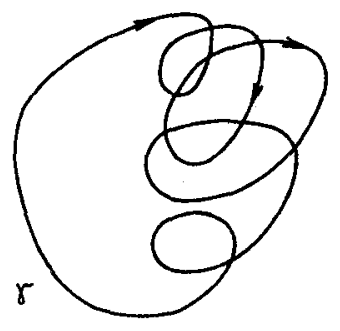
\includegraphics[width=0.30\textwidth]{figures/fig4_21.png}
\par\smallskip
\begin{tabular}{@{}p{0.44\textwidth}p{0.46\textwidth}@{}}
(a) $S^1\to\R^2$，$V^{\R}_{1,2}\sim S^1$，$\pi_1(S^1)\cong\Z$，$\frac{1}{2\pi}\oint_\gamma k\,ds=n$ &
(b) $S^1\to S^2$，$E_{1,2}\cong SO_3$，$\pi_1(SO_3)\cong\Z/2$；于是由 $\R^2$ 转到球面 $S^2$ 时，(a) 中的不变量化为模 $2$ 约化
\end{tabular}
\figtitle{4.21}{}
\end{figure}

关于与球面同伦等价的闭流形的理论，是 Milnor 与 Kervaire 在 1960 年前后建立的。为描述这一理论，需要所谓流形的「连通和」$M^n_1\#M^n_2$ 的构造；关于这个运算，每个维数 $n$ 的光滑流形（的微分同胚类）构成交换半群：从 $M^n_1$、$M^n_2$ 中各挖去一个小圆盘：

% [原文 p.230]
\begin{gather*}
\sum_j(x^j_\alpha)^2<\eps^2\quad \text{在 } M^n_1 \text{ 上},\\
\sum_j(y^j_\beta)^2<\eps^2\quad \text{在 } M^n_2 \text{ 上},
\end{gather*}

这里用的是适当坐标卡 $U_\alpha\subset M^n_1$、$V_\beta\subset M^n_2$ 上的局部坐标；随后把所得边界（每一个都微分同胚于标准球面 $S^{n-1}_\eps$）按标准微分同胚等同起来（若流形带定向，还须计及定向）；所得光滑流形就是\emph{连通和} $M^n_1\#M^n_2$（见图 4.22）。

\begin{figure}[htbp]
\centering
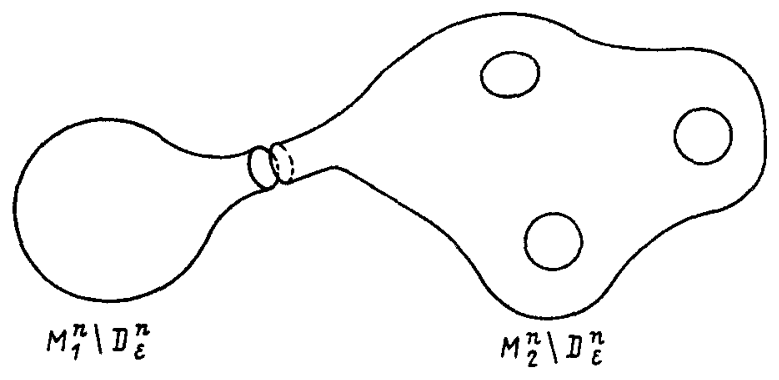
\includegraphics[width=0.55\textwidth]{figures/fig4_22.png}
\figtitle{4.22}{}
\end{figure}

\begin{example*}{}
闭曲面（闭 2 维流形）有完全的分类清单：
\begin{gather*}
M^2_g=\underbrace{T^2\#\cdots\#T^2}_{g\ \text{个}},\qquad T^2 \text{ 为环面},\\
N^2_{1,g}=K^2\#\underbrace{T^2\#\cdots\#T^2}_{g-1\ \text{个}},\qquad K^2 \text{ 为 Klein 瓶},\\
N^2_{2,g}=\RP^2\#\underbrace{T^2\#\cdots\#T^2}_{g\ \text{个}}.
\end{gather*}
于是 $T^2$、$K^2$ 与 $\RP^2$ 是全体闭曲面半群的生成元，定义关系为
\begin{gather*}
\RP^2\#\RP^2\#\RP^2\cong\RP^2\#T^2\cong\RP^2\#K^2,\\
K^2\#T^2\cong K^2\#K^2.
\end{gather*}
（图 4.24、4.25、4.26 图示了这些关系。）
% [Tutor Note: $\Omega_2^O$ 中非零类恰是那些不可定向的闭曲面，即含奇数个交叉帽的曲面：$N^2_{2,g}=\RP^2\#T^2\#\cdots\#T^2$ 正是这样一类。闭曲面半群的生成元 $T^2$、$K^2$、$\RP^2$ 与其关系，可由图 4.25、4.26 直观验证：$K^2\#T^2\cong K^2\#K^2$ 就是把一个把手经曲面拖到外侧、化为两个交叉帽的过程。]
\end{example*}

\begin{figure}[htbp]
\centering
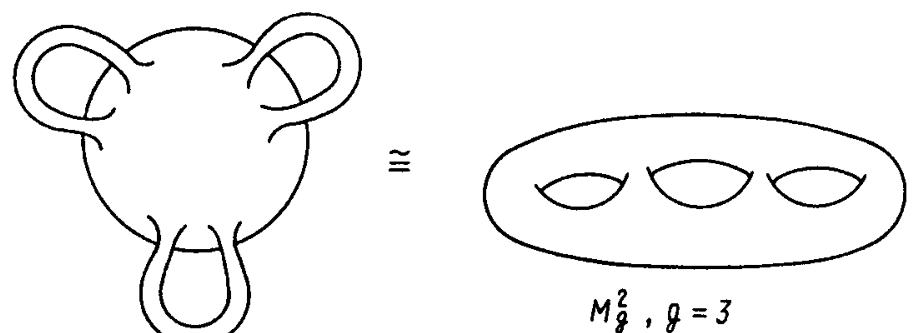
\includegraphics[width=0.62\textwidth]{figures/fig4_23.png}
\figtitle{4.23}{带 $g$ 个把手的球面 $M^2_g$（图中 $g=3$）}
\end{figure}

\begin{remark}{}
可定向闭曲面构成以单个生成元 $T^2$ 为基础的自由幺半群。似乎闭可定向 3-流形也构成
% [原文 p.231]
自由幺半群；不过对闭可定向 4-流形，情况肯定不再如此。顺便注意：在闭曲面中，$N^2_{2,g}$（$g\ge0$）全都代表 $\Omega_2^O$ 中非零的配边类，而其余曲面都代表零类。\hfill$\square$
\end{remark}

\begin{figure}[htbp]
\centering
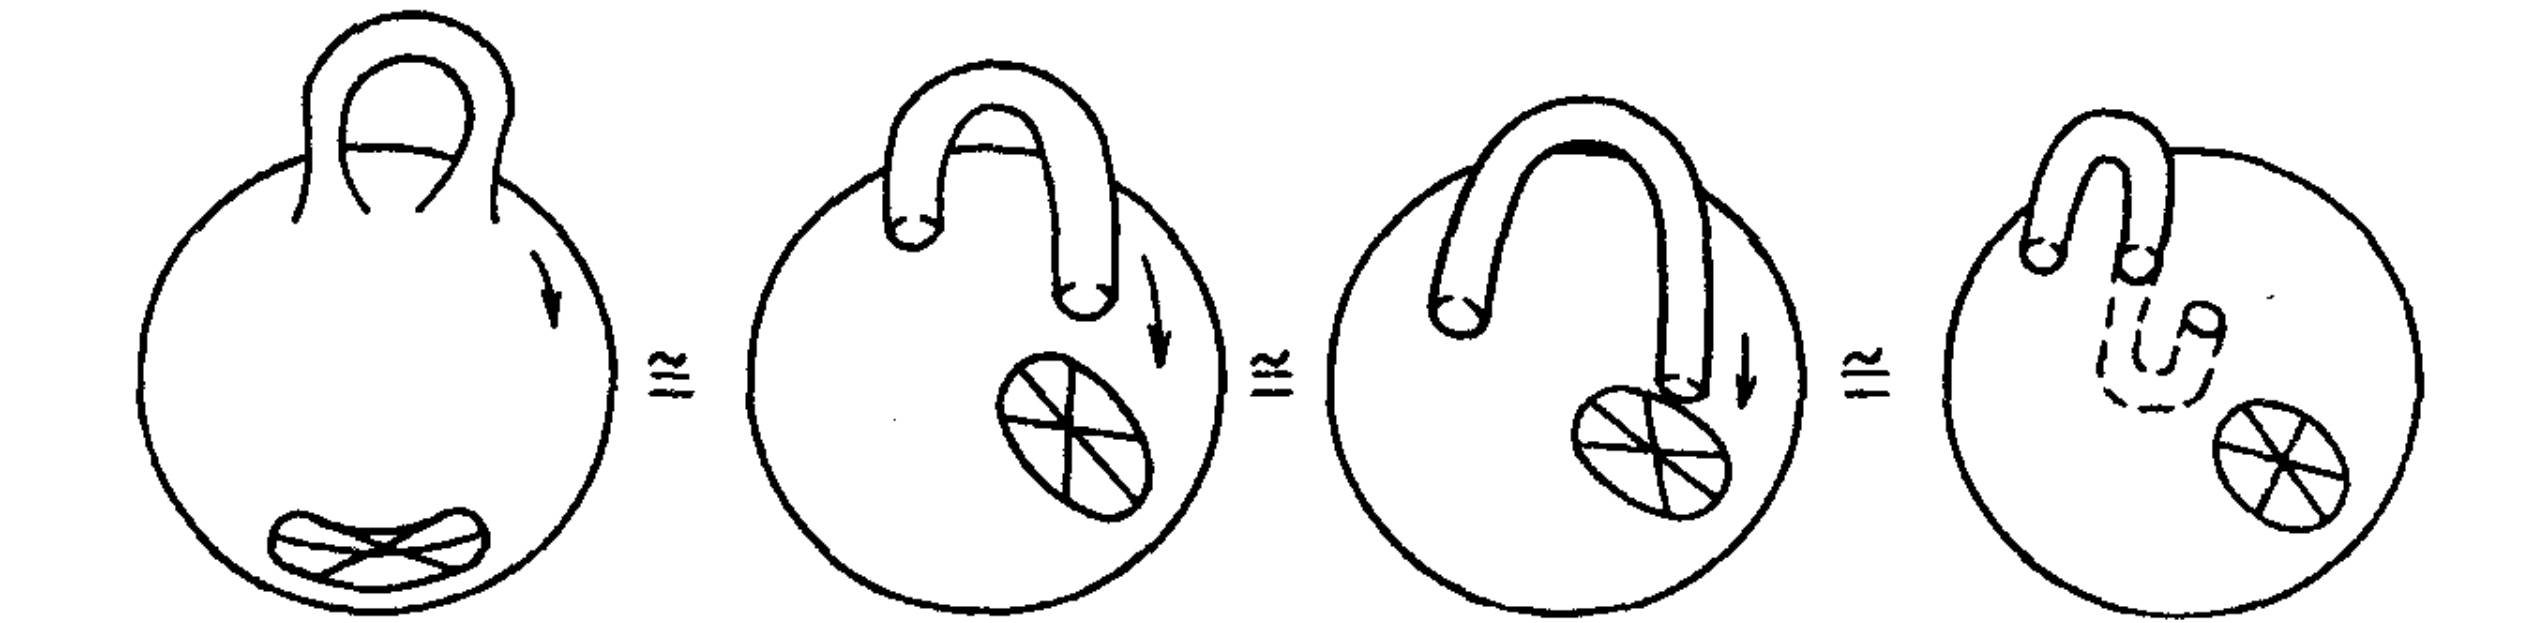
\includegraphics[width=0.85\textwidth]{figures/fig4_24.png}
\figtitle{4.24}{把一个把手从外侧变形到内侧的过程}
\end{figure}

\begin{figure}[htbp]
\centering
\begin{minipage}[t]{0.44\textwidth}
\centering
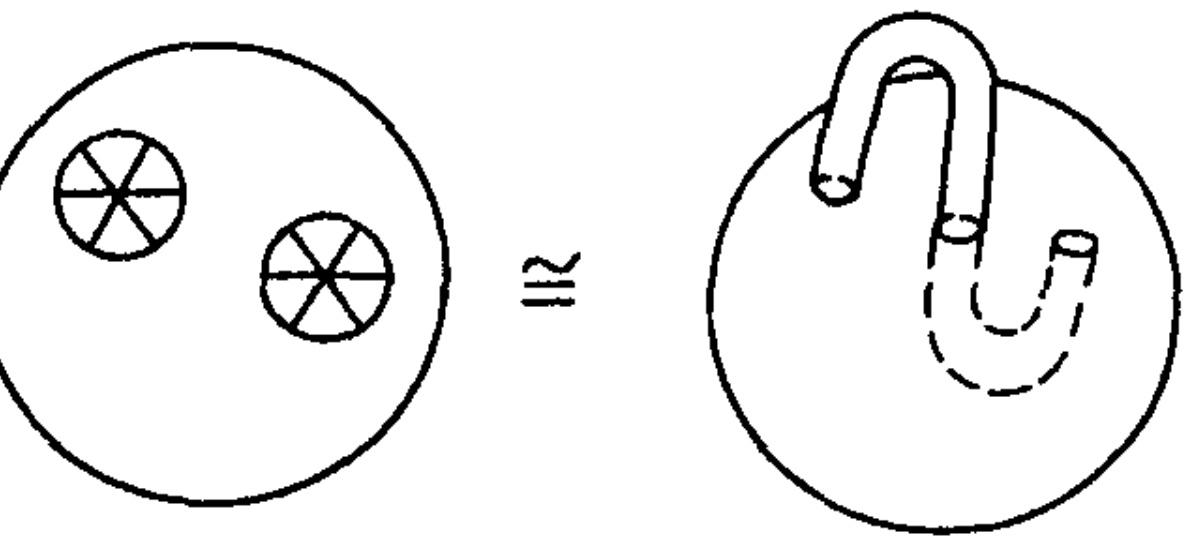
\includegraphics[width=\textwidth]{figures/fig4_25.png}
\figtitle{4.25}{}
\end{minipage}\hfill
\begin{minipage}[t]{0.44\textwidth}
\centering
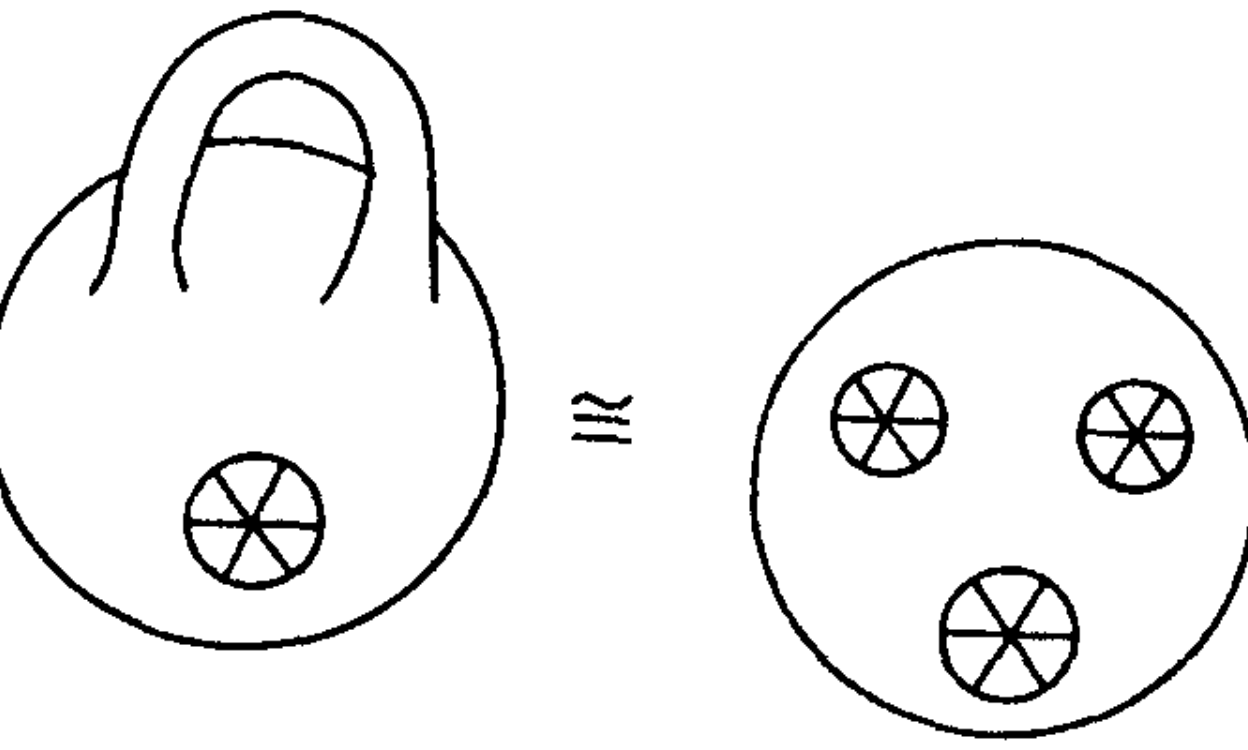
\includegraphics[width=\textwidth]{figures/fig4_26.png}
\figtitle{4.26}{}
\end{minipage}
\end{figure}

现在回到同伦球面。首先注意：同伦 $n$-球面的定向 $h$-配边类在连通和运算下构成一个群（记作 $\Theta^n$）。（$h$-配边的定义见上文 §3。）这里零类由那些是一个可缩带边流形 $W^{n+1}$ 的定向边界的流形 $M^n$ 组成：
\[
M^n=\partial W^{n+1},\qquad W^{n+1}\sim0.
\]
定向同伦 $n$-球面 $M^n_+$ 的类的逆元，就是同一个流形取相反定向后所得的类。为看出这一点，即看出连通和 $M^n_+\#M^n_-$ 与 $S^n$ 是 $h$-配边的，考虑带边流形 $W^{n+1}$，使 $\partial W^{n+1}=M^n_+\#M^n_-$，其构造如下（见图 4.27）：从柱面 $M^n_+\times I$ 中挖去子集 $D^n_\eps\times I$，其中 $D^n_\eps\subset M^n_+$ 是半径为 $\eps$ 的小开球；把角适当「磨光」之后，剩下一个光滑带边流形
\[
W^{n+1}=(M^n_+\times I)\setminus(D^n_\eps\times I)=(M^n_+\setminus D^n_\eps)\times I,
\]
它满足 $\partial W^{n+1}=M^n_+\#M^n_-$，而且还可缩。

% [原文 p.232]
\begin{figure}[htbp]
\centering
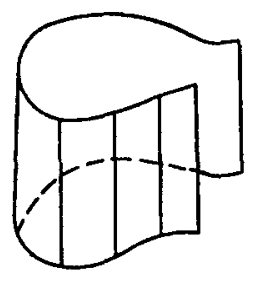
\includegraphics[width=0.24\textwidth]{figures/fig4_27.png}
\figtitle{4.27}{$M^n_+\#M^n_-\sim0$，$M^n\sim S^n$（同伦球面）}
\end{figure}

Smale 的著名「$h$-配边定理」断言：维数 $n\ge5$ 的单连通流形 $M^n_1$、$M^n_2$ 之间的每个 $h$-配边 $W^{n+1}$ 都微分同胚于 $M^n_1\times I$（于是 $M^n_1$ 微分同胚于 $M^n_2$）；由此可知，对每个 $n\ge5$，群 $\Theta^n$ 给出同伦 $n$-球面的精确分类，从而给出拓扑 $n$-球面上可定义的各种光滑结构的精确分类。

% [Tutor Note: 所谓 $\Theta^n$ 给出「拓扑球面上光滑结构」的分类，是因为把同伦球面 $M^n$ 的某个圆盘挖去、换粘标准圆盘，就得到同胚于 $S^n$ 的拓扑流形；$h$-配边定理保证 $n\ge5$ 时同伦球面的微分同胚类恰由 $\Theta^n$ 的元素给出，故 $\Theta^n$ 的大小就是 $S^n$ 上非同胚光滑结构的个数。Rohlin 与 Milnor 的怪球正是 $\Theta^7\cong\Z/28$ 的内容。]

特别令人感兴趣的是 $\Theta^n$ 的子群（记作 $bP^{n+1}$），它由紧可平行化带边流形的边界所成的 $h$-配边类组成。Milnor 证明了如何构造：对每个偶数维、幺模的整数矩阵 $(a_{ij})$（如 (4.4) 所示），可以构造一个可平行化带边流形 $P^{4k}$，其边界为同伦球面 $M^{4k-1}$，且 $H_{2k}(P^{4k};\Z)$ 是以相交指数矩阵为 $(a_{ij})$ 的闭链为基的自由阿贝尔群，并且 $j<2k$ 时 $\tau_j(P^{4k})=0$。这类流形的极小符号差为 $8$：$\tau_{\min}(P^{4k})=8$；下面这个矩阵 $A=(a_{ij})$ 就给出这样的流形：
\begin{equation}
A=\begin{pmatrix}
2&1&0&0&0&0&0&0\\
1&2&1&0&0&0&0&0\\
0&1&2&1&0&0&0&0\\
0&0&1&2&1&0&0&0\\
0&0&0&1&2&1&0&1\\
0&0&0&0&1&2&1&0\\
0&0&0&0&0&1&2&0\\
0&0&0&0&1&0&0&2
\end{pmatrix}. \tag{4.4}
\end{equation}

% [Tutor Note: 原书 p.232 此处作 $\tau_j(P^{4k})=0$；但按 Milnor 的构造，需要的是 $2k$ 维以下的\emph{同伦群}为零（这样手术才能把 $P^{4k}$ 化为 $2k$-连通的，其边界才是同伦球面），故应为 $\pi_j(P^{4k})=0$，正文照排。矩阵 (4.4) 正定、幺模、符号差为 $8$，它就是 $E_8$ 型相交形式；Milnor 用相应的 $P^8$ 造出了 7 维怪球。]

注意，流形 $P^{4k}$ 是 \emph{Spin} 流形（它可定向，且 Stiefel 类 $w_2(P^{4k})=0$）。因此，$P^{4k}$ 的边界是通常的 $(4k-1)$-球面 $S^{4k-1}$ 的一个必要条件是：流形
\[
P^{4k}\cup_{\partial P^{4k}}D^{4k}
\]
的 $A$-亏格为整数（见上文 §3），而该 $A$-亏格由下式给出：

% [原文 p.233]
\[
\hat A\bigl[P^{4k}\cup_{\partial P^{4k}}D^{4k}\bigr]=\tau(P^{4k})\cdot\frac{1}{2^{2k+1}(2^{2k-1}-1)}.
\]
因此在这种情况下，符号差 $\tau(P^{4k})$ 必须实际上被
\[
2^{2k+1}(2^{2k-1}-1)
\]
整除。

利用符号差被 $8$ 整除这一事实，可知群 $bP^{4k}$ 的阶被
\[
2^{2k-2}(2^{2k-1}-1)
\]
整除。

（回忆：$k$ 为偶数时 $\hat A$-亏格也为偶数；因此事实上当 $k$ 为偶数时，群 $bP^{4k}$ 的阶被 $2^{2k-1}(2^{2k-1}-1)$ 整除。）

当 $N$ 充分大（$N>n+1$）时，每个同伦球面 $M^n\subset\R^{n+N}$ 的法丛 $\nu$ 都平凡。（为此要用：$M^n$ 上 $N$-标架法场的分类由 $\pi_n(SO_N)$ 中的元素 $[\nu]$ 给出；$SO$ 的 Bott 周期性；$n=4k$ 时 $p_k(M^n)=0$（这是 Hirzebruch 符号差公式与 $\tau(S^n)=0$ 的推论）；以及 Adams 在 20 世纪 60 年代初的一个结果——它说明在 $\pi_n(SO_N)\cong\Z/2$ 的情形下分类元素 $[\nu]$ 也为零。）由于这一性质，同伦 $n$-球面带标架 $\nu_N$；而 $\R^{n+N}$ 中 $n$-流形上的标架法丛与 $\pi_{N+n}(S^N)$ 的元素之间有一一对应（见上文 §3），其中形如 $(S^n,\nu_N)$ 的标架流形对应于子群 $J(\pi_n(SO_N))$，即 Whitehead 同态下的像（见上文 §3）；于是得到一个同态
\begin{equation}
\mu:\Theta^n\longrightarrow\pi_{N+n}(S^N)/J\pi_n(SO). \tag{4.5}
\end{equation}

这个同态的核，恰为子群 $bP^{n+1}$，即边界可平行化的同伦 $n$-球面的类。Milnor 与 Kervaire 的一个定理断言：只要 $n$ 不具有 $4k+2$ 的形式，同态 $\mu$ 就是满射；而当 $n=4k+2$ 时，$\mu$ 的像的指数至多为 $2$。核 $bP^{n+1}$ 是循环群，且 $n$ 为偶数时实际上是平凡的。进一步已知：对形如 $n=4k+1$ 的 $n$，子群 $bP^{4k+2}\subset\Theta^{4k+1}$ 的阶至多为 $2$；$bP^\infty\cong\Z/28$；并且 $bP^{4k}$ 的阶随 $k\to\infty$ 增大。

为了研究同伦球面，人们发展了一套细致的技术：用「Morse 手术」把标架流形上适当的同伦群「消灭」，使其化为标架同伦球面。（20 世纪 40 年代末 Pontryagin 在 $n=2$ 的情形计算群 $\pi_{n+2}(S^n)$ 时就用了这一技术；见上文 §3。）做法是：先把给定的标架流形换成一个等价的连通标架流形，再换成等价的单连通标架流形，如此继续；需要用非平凡分析处理的困难，只出现在维数 $[n/2]$ 上。$n$ 为奇数时，这一维上不会出现不变量——尽管证明这一点并不平凡。对形如 $n=4k$ 的 $n$，由于标架流形的符号差按 Hirzebruch 公式为零，只要 $n>4$，总可以用初等的 Morse 手术把 $n/2$ 维同伦也消去：此时 $n/2$ 维的闭链可实现为嵌入的 $n/2$-球面，而这正是 Morse 手术所需要的。

% [原文 p.234]
对形如 $n=4k+2$ 的 $n$，标架流形 $M^{4k+2}$ 也可约化为满足「$j\le2k$ 时 $\pi_j(M^{4k+2}_1)=0$」的流形 $M^{4k+2}_1$。此时，$H_{2k+1}(M^{4k+2}_1)\cong\pi_{2k+1}(M^{4k+2}_1)$ 的元素虽如前一情形那样可用嵌入球面 $S^{2k+1}\subset M^{4k+2}_1$ 实现，但这些球面在 $M^{4k+2}_1$ 中的法丛可以非平凡：它对应于第一个非稳定同伦群 $\pi_{2k}(SO_{2k+1})$ 的非平凡元素 $[\nu]$：
\[
[\nu]\in\pi_{2k}(SO_{2k+1})\cong\Z/2,\qquad k\ne0,1,3.
\]
（这些群上文 §2 讨论 Bott 周期性时已经遇到过；那里曾指出：正是它们的非平凡性导致维数 $\ne1,3,7$ 的球面不可平行化，以及维数 $\ne2,4,8$ 的可除代数不存在。）于是，对一切 $k\ne0,1,3$，每个元素
\[
z\in H_{2k+1}(M^{4k+2};\Z)\cong\pi_{2k+1}(M^{4k+2})
\]
对应一个元素
\[
\Phi(z)=[\nu]\in\pi_{2k}(SO_{2k+1})\cong\Z/2,
\]
这就是 \emph{Arf 函数}。Arf 函数 $\Phi$ 满足下面的「Arf 恒等式」
\[
\Phi(z_1+z_2)=\Phi(z_1)+\Phi(z_2)+z_1\circ z_2\pmod2.
\]
对 $k=0,1,3$，Arf 函数还可用球面 $S^{2k+1}\subset M^{4k+2}\subset\R^N$ 上的标架法丛另行定义。（§3 中处理 $k=0$ 的情形时用的正是这一途径。）正如 §3 所述（见那里的 (4.8)），Arf 函数决定了 \emph{Arf 不变量}
\[
\Phi:\pi_{N+4k+2}(S^N)\longrightarrow\Z/2.
\]
「Arf 不变量问题」于是归结为：对各类 $k$ 确定这个同态。在 $k=0,1,3$ 的情形它是非平凡的，作用在稳定群 $\pi_{N+2}(S^N)$、$\pi_{N+6}(S^N)$、$\pi_{N+14}(S^N)$ 上。20 世纪 50 年代末 Kervaire 证明 $k=2$ 时它平凡；由此他构造出一个 10 维 $PL$ 流形，它不同伦等价于任何光滑流形，并证明了 $bP^{10}\cong\Z/2$（$bP^{10}\subset\Theta^9$）。对 $k=0,1,3$，有 $bP^2\cong bP^6\cong bP^{14}\cong\Z/2$。随后 Kervaire 与 Milnor 证明：$\Phi=0$ 当且仅当 $bP^{4k+2}\cong\Z/2$。稍后，20 世纪 60 年代中期，Anderson、Brown 与 Peterson 证明：事实上当 $n=8k+2$ 时，Arf 不变量 $\Phi$ 恒为零；他们的证明用了（Brown 与 Novikov 在 60 年代初提出的）想法——把 Arf 不变量 $\Phi$ 延拓成 $SU$-配边群上的同态：

% [Tutor Note: 原书 p.234 作「$bP^2\cong bP^6\cong bP^{14}\cong\Z/2$」，但 $bP^2\subset\Theta^1=0$，且 $k=0,1,3$ 正是 Arf 不变量非平凡、Kervaire 不变量为 $1$ 的维数；按紧接的 Kervaire--Milnor 定理（$\Phi=0$ 当且仅当 $bP^{4k+2}\cong\Z/2$），此时应有 $bP^2=bP^6=bP^{14}=0$。故此处 $\Z/2$ 疑为 $0$ 之误，正文照排。]

% [原文 p.235]
\[
\pi^S_{8k+2}=\pi_{8k+2+N}(S^N)\longrightarrow\Omega^{SU}_{8k+2}\overset{\Phi}{\longrightarrow}\Z/2.
\]
事实证明，球面同伦群在 $\Omega^{SU}_*$ 中的像可以用相当简单的语言描述，上述结果正由此而来。

对形如 $n=8k+6$ 的 $n$，这条经由普通配边理论的途径行不通。不过，Browder 构造了一种把 Arf 不变量极大延拓的特殊配边理论，从而（在 20 世纪 60 年代末）证明：对一切不具有 $2^s-2$ 形式的 $n$，Arf 不变量 $\Phi$ 为零；对 $n=2^s-2$，它非零当且仅当元素
\[
h^2_{s-1}\in\Ext^{2^s,2}_{A_2}(\Z/2,\Z/2)
\]
关于所有 Adams 微分都是闭链（从而代表群 $\pi_{N+2^s-2}(S^N)$ 的非平凡元素）。特别地，在 $s=5,6$ 的情形，元素 $h^2_4$、$h^2_5$ 确实关于所有 Adams 微分都是闭链，因此 $bP^{30}=0$、$bP^{62}=0$。\footnote{后一结果属于 Barrat、Mahowald 与 J. D. S. Jones；他们在 Adams 谱序列中直接计算，证明了 $h^2_5$ 关于所有 Adams 微分都是闭链。至于 $j\ge6$ 时元素 $h^2_j$ 是否也是闭链，截至 1994 年尚不知道。}

另有一个自然出现的群 $\Gamma^n$，与 $\Theta^n$ 有关：把定向保持微分同胚 $f:S^{n-1}\to S^{n-1}$ 在复合下构成的群 $Diff^+(S^{n-1})$ 的连通分支群，再商掉「可延拓为被 $S^{n-1}$ 所围圆盘 $D^n$ 的微分同胚 $\psi$」的那些 $f$ 所成的正规子群，所得商群就是 $\Gamma^n$：
\[
\psi:D^n\to D^n,\qquad \psi|_{S^{n-1}}=f.
\]
于是有下列同态序列，其复合记作 $\bar\mu$：
\[
\bar\mu:\pi_0(Diff^+(S^{n-1}))\longrightarrow\Gamma^n\longrightarrow\Theta^n\overset{\mu}{\longrightarrow}\pi_{n+N}(S^N)/\Im J.
\]
（这里同态 $\Gamma^n\to\Theta^n$ 这样定义：对每个微分同胚 $f:S^{n-1}_1\to S^{n-1}_2$，配以把两个圆盘 $D^n_1$、$D^n_2$ 的边界按此微分同胚等同起来所得的同伦 $n$-球面。）

由 Smale 的结果可知，$n\ge5$ 时 $\Gamma^n\cong\Theta^n$：因为对这些 $n$，所有同伦球面 $M^n$ 都可由圆盘 $D^n_1$、$D^n_2$ 把边界按某个微分同胚 $f:S^{n-1}_1\to S^{n-1}_2$ 等同而得到。群 $\Gamma^1$、$\Gamma^2$ 的平凡性很容易。$\Gamma^3=0$ 可由 Smale（20 世纪 50 年代末）的结果推出：按该结果，$Diff^+(S^2)$ 同伦等价于 $SO_3$。$\Gamma^4=0$ 则来自 Cerf（20 世纪 60 年代中期）的一个（非常不初等的）结果：$\pi_0(Diff^+(S^3))=1$。另一方面，由 Milnor 的例子（见上文 §3）可知 $\pi_0(Diff^+(S^6))\ne1$。把这些结果（连同其他结果）合起来，得到：
\[
\Gamma^1=\Gamma^2=\Gamma^3=\Gamma^4=\Gamma^5=\Gamma^6=0,
\]
\[
\Gamma^7\cong\Z/28,\qquad \Gamma^n=\Theta^n,\quad n\ne3.
\]
% [Tutor Note: 最后一行把 $n=3$ 排除在外：$\Gamma^3=0$ 已由 $Diff^+(S^2)\simeq SO_3$ 得到，而 $\Theta^3=0$ 等价于 Poincaré 猜想，1994 年时尚未解决；故只能说 $n\ne3$ 时两者相等。$\Gamma^7\cong\Z/28$ 与 $\Theta^7\cong\Z/28$ 一致，正是 28 个 7 维怪球的方向数。]

% [原文 p.236]
纤维丛投影
\begin{equation}
p:Diff^+(D^q)\longrightarrow Diff^+(S^{q-1}), \tag{4.6}
\end{equation}
与包含映射
\[
\kappa:Diff^+(D^q,S^{q-1})\longrightarrow Diff^+(S^q),
\]
都按自然方式定义。纤维丛 (4.6) 的纤维 $F_q$ 是固定边界的微分同胚群：$F_q=Diff^+(D^q,S^{q-1})$。由此得到同伦群的通常诱导同态：
\[
\partial:\pi_j(Diff^+(S^{q-1}))\longrightarrow\pi_{j-1}(Diff^+(D^q,S^{q-1})),
\]
\[
\kappa_*:\pi_{j-1}(Diff^+(D^q,S^{q-1}))\longrightarrow\pi_{j-1}(Diff^+(S^q)).
\]
复合 $2j$ 次，便得到同态
\[
\lambda=(\kappa_*\circ\partial)\circ\cdots\circ(\kappa_*\circ\partial),
\]
\[
\lambda:\pi_j(Diff^+(S^{q-1}))\longrightarrow\pi_0(Diff^+(S^{q+j-1})).
\]
把 $\lambda$ 与 Milnor--Kervaire 同态 $\bar\mu$（见上文）复合：
\[
\bar\mu:\pi_0(Diff^+(S^{q-1}))\longrightarrow\pi_{q+N}(S^N)/\Im J\pi_q(SO_N),
\]
可以证明下面的公式在球面稳定同伦环中（或在标架流形的配边环 $\Omega^{Fr}_*$ 中）成立，对一切元素 $a\in\pi_0(Diff^+(S^{N-1}))$、$b\in\pi_q(SO_N)$：
\begin{equation}
\bar\mu(\lambda(aba^{-1}))=\bar\mu(a)\circ J(b)\pmod{J\pi_{q+N}(SO_N)}, \tag{4.7}
\end{equation}
\[
aba^{-1}\in\pi_q(Diff^+(S^{N-1})).
\]
在某些维数上，环
\[
\Omega^{Fr}_*=\sum_{j\ge0}\pi_{N+j}(S^N)
\]
的结构使得 (4.7) 的右端（对适当的 $a,b$）不为零；例如 $q=1$、$n=8$ 时就是如此——见第 3 章 §7 末的表。由此可以推断：对这些 $N$，空间 $Diff^+(S^{N-1})$ 的单位元连通分支不能收缩到子群 $SO_N$ 上（Novikov，20 世纪 60 年代初）。\footnote{稍后 Milnor 也独立证明了这一结果。}

闭的、单连通 $n$ 维流形（$n\ge5$）的一般分类理论，以及随后非单连通流形的分类理论，都依赖于闭流形之间度数为 $1$ 的映射
% [原文 p.237]
\[
f:M^n_1\longrightarrow M^n_2
\]
的某些重要而初等的性质。对这类（度数为 $1$ 的）映射，同态 $f_*D^{-1}f^*D$（其中 $D$ 是 Poincaré 对偶同构）是 $M^n_1$ 的同调上的恒等映射，因此同调有标准的分解
\begin{equation}
H_*(M_1)\cong(D^{-1}f^*D)(H_*(M_2))\oplus\Ker f_*, \tag{4.8}
\end{equation}
它关于闭链的相交是正交的（对 $M^n_1$ 的上同调也类似）。同调的这个直和项 $\Ker f_*$ 在 Poincaré 对偶算子下封闭，一般表现得就像它自身代表某个流形的同调。于是，若第 $j$ 个同伦群的诱导映射 $f^{(\pi_j)}_*$ 的核 $\Ker f^{(\pi_j)}_*\subset\pi_j(M^n_1)$ 在 $j<k-1$ 时平凡，则对第 $k$ 个这样的核，Hurewicz 定理的类似物成立：
\begin{equation}
\Ker f^{(\pi_k)}_*\cong\Ker f^{(H_k)}_*, \tag{4.9}
\end{equation}
并且相应同伦群之间的诱导同态
\[
f_*:\pi_i(M^n_1)\longrightarrow\pi_i(M^n_2)
\]
在 $i<k$ 时是同构。对非单连通流形，只要把同调群看成 $\Z[\pi]$-模（其中 $\pi_1(M^n_1)\cong\pi_1(M^n_2)\cong\pi$），这一结果依然成立。在与前面相同的假设下，即诱导同态在 $\pi_i$ 上的核在 $i<k-1$ 时平凡，有同构
\begin{equation}
\Ker f^{(H_k)}_*\cong\Ker f^{(\pi_k)}_*\otimes_{\Z[\pi]}\Z \tag{4.10}
\end{equation}
（这里要求基本群 $\pi_1$ 的诱导同态的核平凡）。

给定同伦型的流形的分类理论，是 Novikov 在 20 世纪 60 年代初建立的；而闭光滑流形全部同伦型的分类理论，则由 Browder 与 Novikov（同样在 60 年代初）建立。在解决这些分类问题的过程中，会遇到这样的情形：流形的某个同伦型由特定的 $CW$-复形 $X$ 代表。在最一般的情形（按 Browder 的表述），$X$ 不必是流形，其几何维数也可以不同于给定的 $n$；只要求存在基本类 $[X^n]\in H_n(X^n;\Z)$，使上积运算 $a\mapsto a\cap[X^n]$ 给出从同调到上同调的适当 Poincaré 同构；具有这一性质的 $CW$-复形称为\emph{Poincaré 复形}。原来，Poincaré 复形 $X$ 具有唯一的稳定「法球丛」$\nu_X$，其行为像流形的通常稳定法丛；当 $X$ 是光滑（或 $PL$）流形时，$\nu_X$ 就是其标准法丛的稳定同伦类。若存在同伦等价 $f:M^n\to X$，其中 $M^n$ 是流形，则必存在 $X$ 上的向量丛 $\xi$，它与稳定法球丛 $\nu_X$ 同伦等价（若 $g:X\to M^n$ 是 $f$ 的同伦逆，则 $\xi=g^*\nu_M$）。

% [原文 p.238]
于是上面的分类问题归结为：考虑 Poincaré 复形 $X$ 连同 $X$ 上与稳定法球丛 $\nu_X$ 同伦等价的向量丛 $\xi$。不过当 $X$ 是光滑闭流形时，向量丛 $\xi$ 与通常法丛 $\nu_X$ 同伦等价；而在这种向量丛 $\xi$ 中确定自由度的任务，可以有效地解决（Novikov，20 世纪 60 年代初）。

设给定 Poincaré 复形 $X$ 上有向量丛 $\xi$。度数为 $1$ 的映射 $f:M^n\to X$ 称为\emph{法映射}（normal map），如果法丛 $\nu_M$ 与 $f^*\xi$（作为向量丛）等价，即有交换图：
\begin{equation}
\begin{tikzpicture}[>=Stealth,baseline=(current bounding box.center)]
\node (a) at (0,1.15) {$\nu_M$};
\node (b) at (2.2,1.15) {$\xi$};
\node (c) at (0,0) {$M$};
\node (d) at (2.2,0) {$X$};
\draw[->] (a)--(b) node[midway,above] {$f$};
\draw[->] (a)--(c);
\draw[->] (b)--(d);
\draw[->] (c)--(d) node[midway,below] {$f$};
\end{tikzpicture} \tag{4.11}
\end{equation}

在这种情形下，核 $\Ker f_*$ 无论对同调还是对同伦，其表现都与可平行化流形的情形相同；这就允许使用 Milnor--Kervaire 技术的自然类比，用 Morse 手术把诱导同伦群映射的核消去。给定流形（更一般地，给定 Poincaré 复形）$X^n$ 及 $X^n$ 上的向量丛 $\xi$，可以定义法映射 $f:M^n\to X^n$（$f^*\xi=\nu_M$）的法配边类，其中法映射被丛映射 $\hat f:\nu_M\to\xi$ 覆盖，$\nu_M$ 是 $M^n\subset\R^{n+N}$ 的稳定法丛；定义如下：\emph{法配边}（normal bordism）是被丛映射 $\hat g$ 覆盖的法映射 $g$，如下图所示：
\begin{equation}
\begin{tikzpicture}[>=Stealth,baseline=(current bounding box.center)]
\node (a) at (0,1.15) {$\nu_N$};
\node (b) at (2.8,1.15) {$\xi\times\eps^0$};
\node (c) at (0,0) {$N^{n+1}$};
\node (d) at (2.8,0) {$X^n\times I$};
\draw[->] (a)--(b) node[midway,above] {$\hat g$};
\draw[->] (a)--(c);
\draw[->] (b)--(d);
\draw[->] (c)--(d) node[midway,below] {$g$};
\end{tikzpicture} \tag{4.12}
\end{equation}
其中流形 $N^{n+1}\subset\R^{n+N}\times I$，$I=[a,b]$，它横截地逼近 $\R^{n+N}\times I$ 的边界，并且自身以
\[
\partial N^{n+1}=M^n_a\cup M^n_b,
\]
\[
M^n_a\subset\R^{n+N}\times\{a\},\qquad M^n_b\subset\R^{n+N}\times\{b\},
\]
为边界，在其每个分支上都给定了度数为 $1$ 的法映射。所得配边类的集合记作 $\mathcal{N}(X^n,\xi)$。可以证明（这并不困难）：集合 $\mathcal{N}(X^n,\xi)$ 可实现为同伦群 $\pi_{n+N}(T\xi)$（丛 $\xi$ 的 Thom 空间）中那些与基本类 $[X^n]$ 同调的元素 $\alpha$ 所成的子集（见上文），即满足
\begin{equation}
H(\alpha)=\phi[X^n]\in H_{n+N}(T\xi)\cong\Z \tag{4.13}
\end{equation}
的元素 $\alpha$；其中
\[
H:\pi_j(T\xi)\longrightarrow H_j(T\xi;\Z)
\]
是 Hurewicz 同态，而 $\phi:H_n(X^n;\Z)\to H_{n+N}(T\xi;\Z)$ 是 Thom 同构。

% CHUNK ch04h DONE
